% TODO

\begin{figure}[htbp]
    \centering
    \makebox[\textwidth][c]{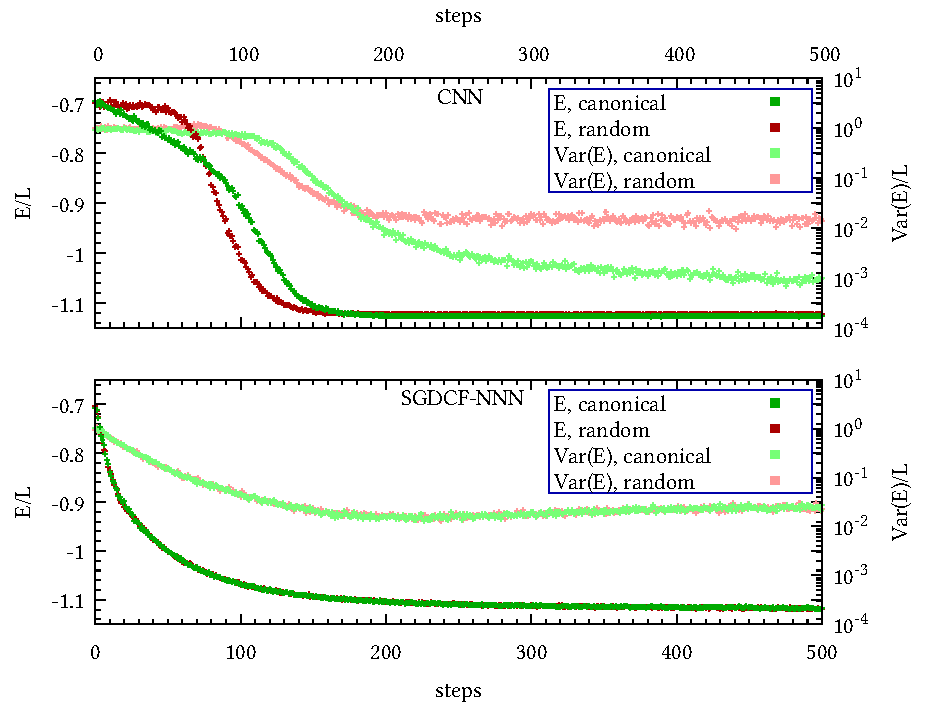
\includegraphics[width=1\textwidth]{./experiments/ground-state-search/resiliency-encoding/encoding-comparison/encoding-comparison.pdf}}
    \caption{
        Visualization of the reaction of a CNN and a SGDCF-NNN network to a change in lattice encoding.
        The calculations are performed for a transverse field Ising model with $J = -1$, $h=-0.7$ on a 1D-linear lattice chain.
        The SGDCF-NNN has a depth of 1, an embed dimension of 16 and a mlp-ratio of 2, making both models have approximately the same number of parameters (CNN: 1280, SGDCF-NNN: 1312).
        The canonical numbering for the lattice sites is printed in green, while the random numbering and therefore unstructured representation in memory is pictured red. 
        The variance is pictured in the same graph, colored in the respective light shade.
    }
    \label{fig:resiliency-encoding}
\end{figure}